\section{Real-world experiment}
\label{sec:real}
\begin{figure*}[t]
\centering
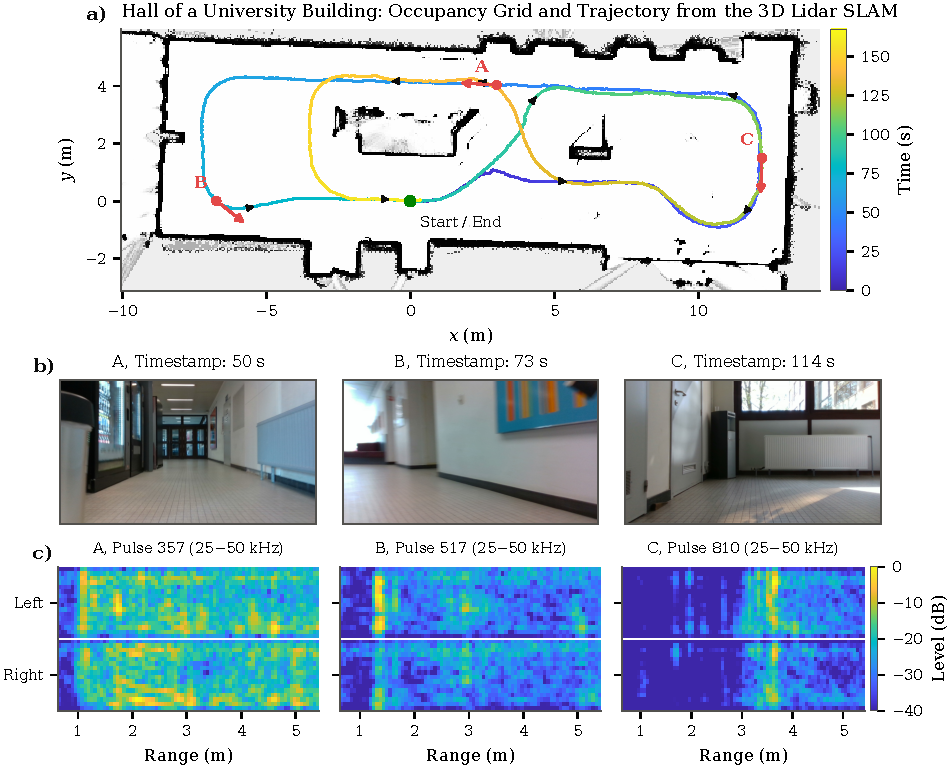
\includegraphics[width=\linewidth]{figures/real_world.pdf}
\caption{The real-world recording. a) Occupancy grid of the hall from the lidar scans, with the ground-truth trajectory (colored by time); the left loop was driven twice in the same direction, the right loop once in each direction. b) Camera images at places A, B and C. c) Binaural cochleograms of the closest sonar pulse, formed with the virtual ears of equation \ref{eq:ears}.}
\label{fig:realWorld}
\end{figure*}

In this section, we apply BatSLAM 2.0 to a real recording. As no binaural bat-head sonar recording of a suitable drive was available, we used an embedded 3D sonar sensor (eRTIS \cite{kerstensERTISFullyEmbedded2019}), and formed two virtual ears from its microphone array. Apart from the virtual ears and the frequency band, the system is identical to the one of the previous sections.

\subsection{Recording, virtual ears and ground truth}
\label{sec:realSetup}
\textbf{Recording:} The eRTIS sensor was mounted on a mobile platform together with a 3D lidar (Ouster OS0) and a camera, and driven through a hall of \SI{22}{\meter} by \SI{8}{\meter} in a university building (figure \ref{fig:realWorld}). The drive is a figure-eight of \RealDist{}~\si{\meter}, during which the sensor emitted \RealPulses{} calls at about \RealRateHz{}~\si{\hertz}. The call is a \SI{2.5}{\milli\second} FM downsweep from \SI{50}{\kilo\hertz} to \SI{25}{\kilo\hertz}, recorded by 32 MEMS microphones in a pseudo-random planar array of about \SI{7}{\centi\meter} by \SI{4}{\centi\meter}. We used the ranges between \SI{0.6}{\meter} and \SI{5.5}{\meter}.

\textbf{Virtual ears:} We split the array into a left and a right half of 16 microphones each, and steered each half with a delay-and-sum beamformer towards an azimuth of \SI{30}{\degree} to its own side:
\begin{equation}
\begin{aligned}
s_L(t) &= \sum_{i \in \mathcal{L}} w_i \, x_i\!\left(t + \frac{y_i \sin 30^\circ}{c}\right), \\
s_R(t) &= \sum_{i \in \mathcal{R}} w_i \, x_i\!\left(t - \frac{y_i \sin 30^\circ}{c}\right),
\end{aligned}
\label{eq:ears}
\end{equation}
with $x_i(t)$ the signal of microphone $i$, $y_i$ its lateral position, $\mathcal{L}$ and $\mathcal{R}$ the two halves, and $w_i$ a Gaussian taper. As the aperture of each half spans between two and a half and five wavelengths over the band of the call, the beams are wide at \SI{25}{\kilo\hertz} and narrow at \SI{50}{\kilo\hertz}, which gives the virtual ears a frequency-dependent directivity, similar to the HRTF characteristics of the real bats used in simulation. As the call covers only one octave, we used 16 pooled channels between \SI{25}{\kilo\hertz} and \SI{50}{\kilo\hertz}.

\textbf{Ground truth and odometry:} The ground truth was computed from the lidar scans with PIN-SLAM \cite{panPINSLAMLiDARSLAM2024}, and the clock offset between sonar and lidar was estimated by comparing the acoustic images with images predicted from the lidar map. As the platform recorded no wheel odometry, we derived it from the ground truth with a scale error of \SI{-5}{\percent} on distance and \SI{+10}{\percent} on rotation, plus the random noise of the simulations. On a figure-eight, the rotation error does not cancel, and at the first revisit, the heading is off by \SI{36}{\degree}. Dead reckoning has an error of \RealATEodo{}~\si{\meter}, and all results are the mean (standard deviation) over ten noise seeds.

\subsection{Results}
\label{sec:realResults}

\begin{figure*}[t]
\centering
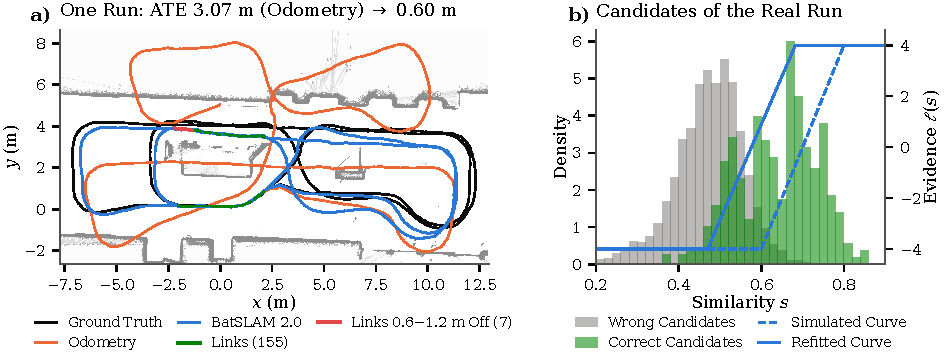
\includegraphics[width=\linewidth]{figures/real_results.pdf}
\caption{Real-world results. a) Map of one run (refitted evidence curve) with odometry, ground truth, BatSLAM 2.0 estimate and links. b) Similarity of correct and wrong candidates, with the simulated (dashed) and refitted (solid) evidence curves.}
\label{fig:realResults}
\end{figure*}

\textbf{The evidence curve:} The real similarities $s$ (equation \ref{eq:similarity}) are lower than the simulated ones. The correct candidates had a median similarity of \RealSimTrueMed{}, and \SI{99}{\percent} of the wrong ones stayed below \RealSimFalsePnn{} (figure \ref{fig:realResults}b). Both classes are well separated, but the evidence curve of the simulations (equation \ref{eq:evidenceCurve}, with its zero crossing at \LLRmid{}) lies above most correct matches. A correct pair with the median similarity then contributes $\ell = \LLRslope \cdot (\RealSimTrueMed - \LLRmid) = -2$ to the evidence $\Lambda(h)$ of equation \ref{eq:evidence}, so that a hypothesis of typical correct pairs loses evidence with every pulse instead of gaining it, and only stretches with similarities above \LLRmid{} can reach the commit threshold. We therefore refitted the two constants of equation \ref{eq:evidenceCurve} with the same logistic regression as in the simulations (equation \ref{eq:llr}), on the candidates of one half of the drive (alternating stretches of \SI{5}{\meter}), labeled with the lidar ground truth, and ran the complete drive with it. Both folds gave similar curves (a zero crossing at \RealMidEven{} and \RealMidOdd{}). This curve is a property of the sensor, and has to be determined once per sensor rather than per deployment.

\textbf{The map:} Table \ref{tab:real} in the appendix and figure \ref{fig:realResults}a summarize the results. With either evidence curve, none of the 30 runs committed a wrong hypothesis or collapsed. With the curve of the simulations, the system linked only half of the revisits, and reduced the trajectory error from \RealATEodo{}~\si{\meter} to \RealATESim{}~\si{\meter}. With the refitted curve, it linked \RealCovEven{} of the revisits and reached \RealATEEven{}~\si{\meter} (\RealATEalEven{}~\si{\meter} after alignment). The remaining error stems mostly from the first \SI{46}{\meter} of the drive, before the first same-direction revisit. Places in the right loop were only revisited in the opposite direction, and were, as expected, never linked. With the refitted curve, a few links (\RealWrongLinksEven{} per run on average) at the tail of one correct hypothesis were \SI{0.6}{\meter} to \SI{1.2}{\meter} off, at a place where the platform turned off a path that it had previously driven straight on. The long-baseline tolerance of the verifier allows such a slow divergence.

\textbf{Odometry errors:} With a rotation error of \SI{15}{\percent} instead of \SI{10}{\percent}, the heading error at the first revisit grows to \SI{53}{\degree}, which the plausibility gate considers implausible given the heading noise assumed by the back-end. The correct loop closures are then rejected (\RealATEcliffEven{}~\si{\meter}), but no wrong loop closure is committed either, and with twice the assumed heading noise, the system recovers (\RealATEcliffNoise{}~\si{\meter}). Finally, the system runs in real time on this drive, with \RealFrontendMs{}~\si{\milli\second} for the front-end and \RealSlamMs{}~\si{\milli\second} for the rest of the system per pulse on average, against \RealBudgetMs{}~\si{\milli\second} between two calls.
